\documentclass{article}
\usepackage{graphicx}
\usepackage{titlesec}
\usepackage{float}
\usepackage[export]{adjustbox}

\setcounter{secnumdepth}{4}

\begin{document}

    \title{Processor Design}
    \author{Spencer Melnick}

    \maketitle

    \section{Introduction}

    \section{Modules}

    \subsection{Adder}

    The adder used in this processor is a simple 32 bit ripple-carry adder.
    The 32 bit adder is created using a series of smaller adder modules
    including:
    
    \begin{itemize}
        \item Half Adder
        \item Full Adder
        \item 2 Bit Adder
        \item 4 Bit Adder
        \item 16 Bit Adder
        \item 32 Bit Adder
    \end{itemize}



    % Half Adder Module

    \subsubsection{Half Adder}

    \paragraph{Inputs}
    \begin{itemize}
        \item Operand A - 1 bit
        \item Operand B - 1 bit
    \end{itemize}

    \paragraph{Outputs}
    \begin{itemize}
        \item Sum - 1 bit
        \item Carry - 1 bit
    \end{itemize}

    \paragraph{Functionality}
    \hfill\\\\
    Takes two single bit operands and produces the single bit sum and the
    carry bit.

    \paragraph{Diagrams}
    \hfill\\\\
    \begin{figure}[H]
        \centering
        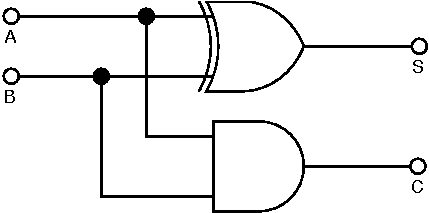
\includegraphics{../diagrams/alu/adder/half_adder.pdf}
        \caption{Logic diagram of the half adder}
    \end{figure}

    \paragraph{Testing}
    \hfill\\\\
    All possible inputs for the half adder are stimulated by the test bench
    and are compared to the expected outputs according to the following
    table:

    \hfill\\
    \begin{tabular}{|c|c||c|c|}
        \hline
        A & B & S & C
        \\\hline\hline
        0 & 0 & 0 & 0
        \\\hline
        1 & 0 & 1 & 0
        \\\hline
        0 & 1 & 1 & 0
        \\\hline
        1 & 1 & 0 & 1
        \\\hline
    \end{tabular}

    \begin{figure}[H]
        \centering
        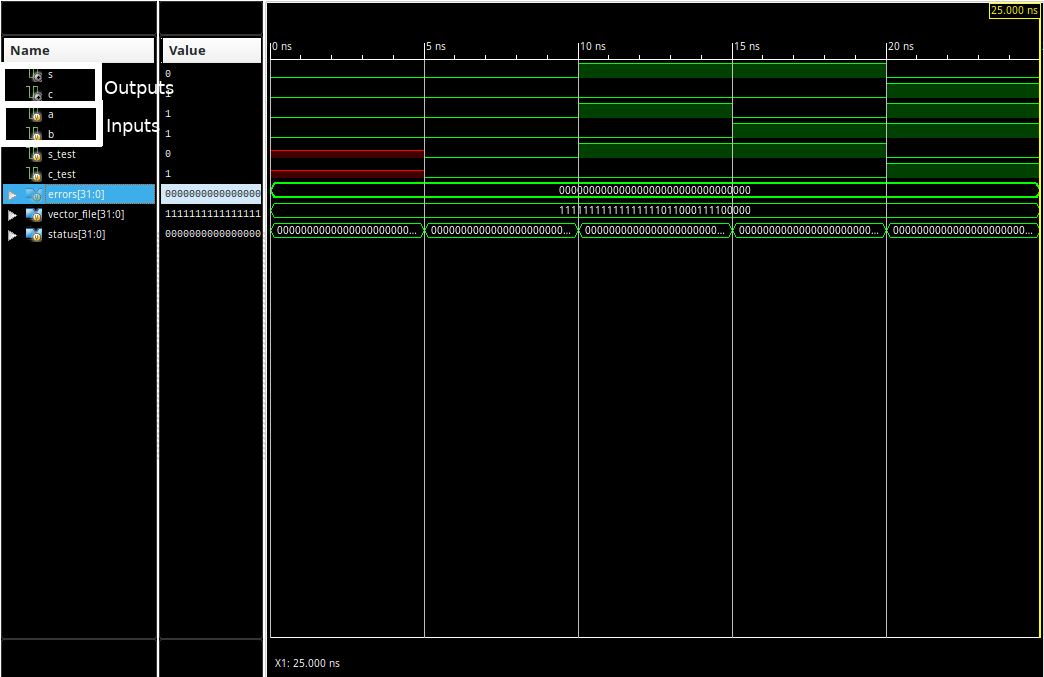
\includegraphics[width=0.9\paperwidth,center]{Screenshots/half_adder.png}
        \caption{Simulation output of half adder}
    \end{figure}



    % Full Adder Module

    \subsubsection{Full Adder}

    \paragraph{Inputs}
    \begin{itemize}
        \item Operand A - 1 bit
        \item Operand B - 1 bit
        \item Carry In - 1 bit
    \end{itemize}

    \paragraph{Outputs}
    \begin{itemize}
        \item Sum - 1 bit
        \item Carry Out - 1 bit
    \end{itemize}

    \paragraph{Functionality}
    \hfill\\\\
    Takes three single bit operands and produces the single bit sum and the
    carry bit.

    \paragraph{Diagrams}
    \hfill\\\\
    \begin{figure}[H]
        \centering
        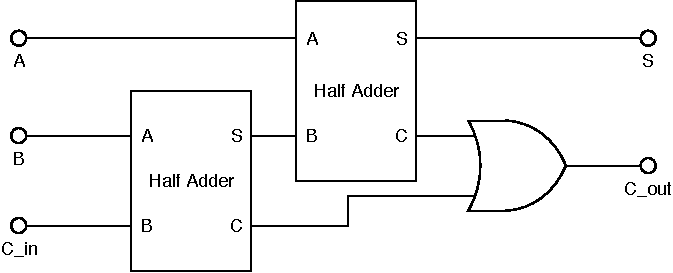
\includegraphics{../diagrams/alu/adder/full_adder.pdf}
        \caption{Logic diagram of the full adder}
    \end{figure}

    \paragraph{Testing}
    \hfill\\\\
    All possible inputs for the full adder are stimulated by the test bench
    and are compared to the expected outputs according to the following
    table:

    \hfill\\
    \begin{tabular}{|c|c|c||c|c|}
        \hline
        A & B & Carry In & S & Carry Out
        \\\hline\hline
        0 & 0 & 0 & 0 & 0
        \\\hline
        1 & 0 & 0 & 1 & 0
        \\\hline
        0 & 1 & 0 & 1 & 0
        \\\hline
        1 & 1 & 0 & 0 & 1
        \\\hline
        0 & 0 & 1 & 1 & 0
        \\\hline
        1 & 0 & 1 & 0 & 1
        \\\hline
        0 & 1 & 1 & 0 & 1
        \\\hline
        1 & 1 & 1 & 1 & 1
        \\\hline
    \end{tabular}

    \begin{figure}[H]
        \centering
        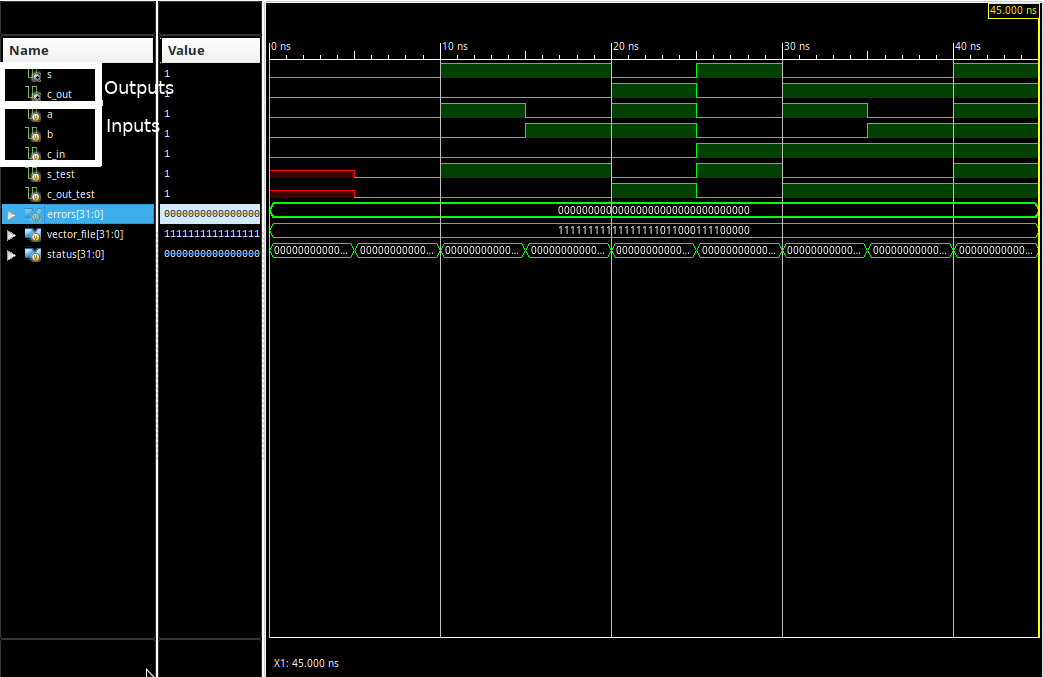
\includegraphics[width=0.9\paperwidth,center]{Screenshots/full_adder.png}
        \caption{Simulation output of full adder}
    \end{figure}



    % 2 Bit Adder Module

    \subsubsection{2 Bit Adder}

    \paragraph{Inputs}
    \begin{itemize}
        \item Operand A - 2 bit
        \item Operand B - 2 bit
        \item Carry In - 1 bit
    \end{itemize}

    \paragraph{Outputs}
    \begin{itemize}
        \item Sum - 2 bit
        \item Carry Out - 1 bit
    \end{itemize}

    \paragraph{Functionality}
    \hfill\\\\
    Takes two 2 bit operands and a third single bit operand and produces the
    2 bit sum and the carry bit.

    \paragraph{Diagrams}
    \hfill\\\\
    \begin{figure}[H]
        \centering
        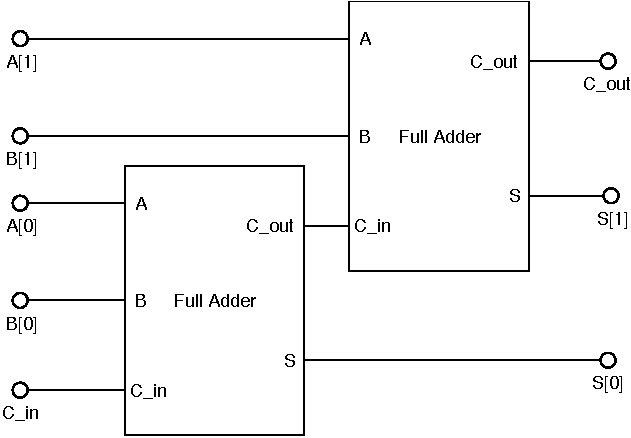
\includegraphics{../diagrams/alu/adder/adder_2.pdf}
        \caption{Logic diagram of the 2 bit adder}
    \end{figure}

    \paragraph{Testing}
    \hfill\\\\
    Due to the larger range of possible inputs, inputs are selected to include
    several base cases, as well as the maximum input value case and minimum
    input value case. The inputs and expected outputs are as follows:

    \hfill\\
    \begin{tabular}{|c|c|c||c|c|}
        \hline
        A & B & Carry In & S & Carry Out
        \\\hline\hline
        3 & 3 & 0 & 2 & 1
        \\\hline\hline
        3 & 1 & 0 & 0 & 1
        \\\hline\hline
        3 & 3 & 1 & 3 & 1
        \\\hline\hline
        0 & 0 & 0 & 0 & 0
        \\\hline
    \end{tabular}

    \begin{figure}[H]
        \centering
        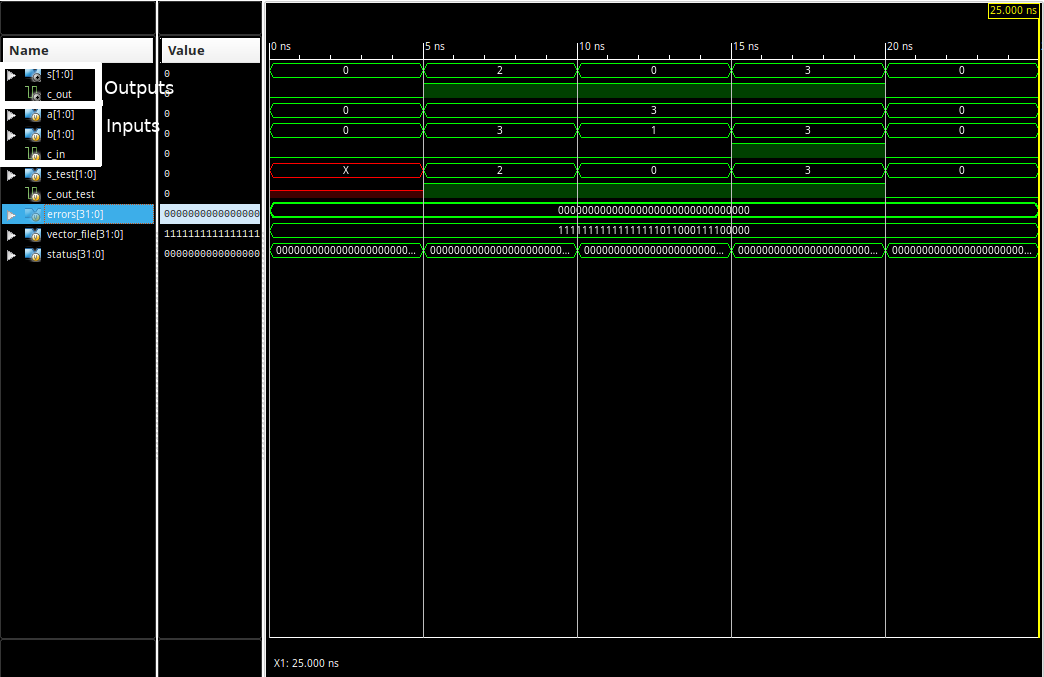
\includegraphics[width=0.9\paperwidth,center]{Screenshots/adder_2.png}
        \caption{Simulation output of 2 bit adder}
    \end{figure}



       % 4 Bit Adder Module

       \subsubsection{4 Bit Adder}

       \paragraph{Inputs}
       \begin{itemize}
           \item Operand A - 4 bit
           \item Operand B - 4 bit
           \item Carry In - 1 bit
       \end{itemize}
   
       \paragraph{Outputs}
       \begin{itemize}
           \item Sum - 4 bit
           \item Carry Out - 4 bit
       \end{itemize}
   
       \paragraph{Functionality}
       \hfill\\\\
       Takes two 4 bit operands and a third single bit operand and produces the
       4 bit sum and the carry bit.
   
       \paragraph{Diagrams}
       \hfill\\\\
       \begin{figure}[H]
           \centering
           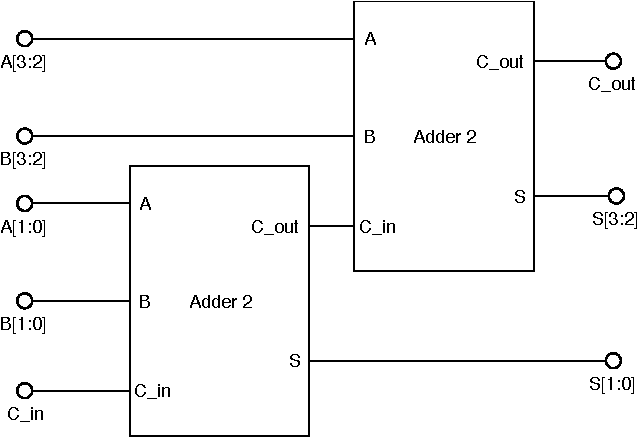
\includegraphics{../diagrams/alu/adder/adder_4.pdf}
           \caption{Logic diagram of the 4 bit adder}
       \end{figure}
   
       \paragraph{Testing}
       \hfill\\\\
       As this module follows a nearly identical functionality as the 2
       bit adder, and nearly identical Verilog code, testing was ommitted.
       This module's test is included within the 32 bit adder test, as the
       32 bit adder will only function correctly if this module functions
       correctly.




       % 8 Bit Adder Module

       \subsubsection{8 Bit Adder}

       \paragraph{Inputs}
       \begin{itemize}
           \item Operand A - 8 bit
           \item Operand B - 8 bit
           \item Carry In - 1 bit
       \end{itemize}
   
       \paragraph{Outputs}
       \begin{itemize}
           \item Sum - 8 bit
           \item Carry Out - 8 bit
       \end{itemize}
   
       \paragraph{Functionality}
       \hfill\\\\
       Takes two 8 bit operands and a third single bit operand and produces the
       8 bit sum and the carry bit.
   
       \paragraph{Diagrams}
       \hfill\\\\
       \begin{figure}[H]
           \centering
           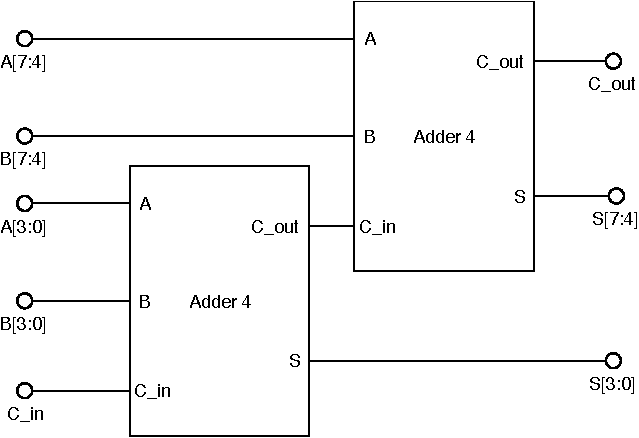
\includegraphics{../diagrams/alu/adder/adder_8.pdf}
           \caption{Logic diagram of the 8 bit adder}
       \end{figure}
   
       \paragraph{Testing}
       \hfill\\\\
       As this module follows a nearly identical functionality as the 2
       bit adder, and nearly identical Verilog code, testing was ommitted.
       This module's test is included within the 32 bit adder test, as the
       32 bit adder will only function correctly if this module functions
       correctly.
    
    


       % 16 Bit Adder Module

       \subsubsection{16 Bit Adder}

       \paragraph{Inputs}
       \begin{itemize}
           \item Operand A - 16 bit
           \item Operand B - 16 bit
           \item Carry In - 1 bit
       \end{itemize}
   
       \paragraph{Outputs}
       \begin{itemize}
           \item Sum - 16 bit
           \item Carry Out - 16 bit
       \end{itemize}
   
       \paragraph{Functionality}
       \hfill\\\\
       Takes two 16 bit operands and a third single bit operand and produces the
       16 bit sum and the carry bit.
   
       \paragraph{Diagrams}
       \hfill\\\\
       \begin{figure}[H]
           \centering
           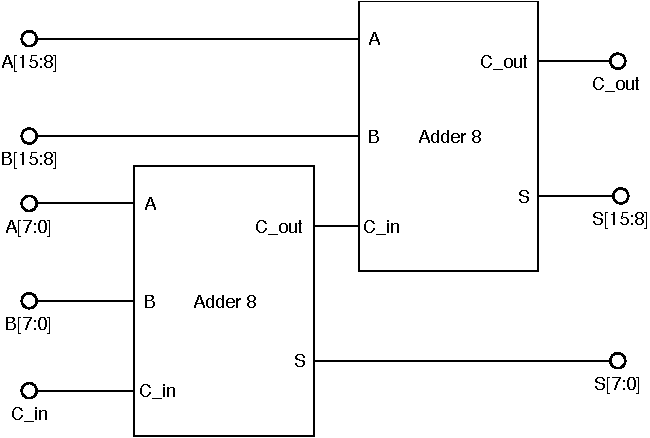
\includegraphics{../diagrams/alu/adder/adder_16.pdf}
           \caption{Logic diagram of the 16 bit adder}
       \end{figure}
   
       \paragraph{Testing}
       \hfill\\\\
       As this module follows a nearly identical functionality as the 2
       bit adder, and nearly identical Verilog code, testing was ommitted.
       This module's test is included within the 32 bit adder test, as the
       32 bit adder will only function correctly if this module functions
       correctly.



    % 32 Bit Adder Module

    \subsubsection{32 Bit Adder}

    \paragraph{Inputs}
    \begin{itemize}
        \item Operand A - 32 bit
        \item Operand B - 32 bit
        \item Carry In - 1 bit
    \end{itemize}

    \paragraph{Outputs}
    \begin{itemize}
        \item Sum - 32 bit
        \item Carry Out - 32 bit
    \end{itemize}

    \paragraph{Functionality}
    \hfill\\\\
    Takes two 32 bit operands and a third single bit operand and produces the
    32 bit sum and the carry bit.

    \paragraph{Diagrams}
    \hfill\\\\
    \begin{figure}[H]
        \centering
        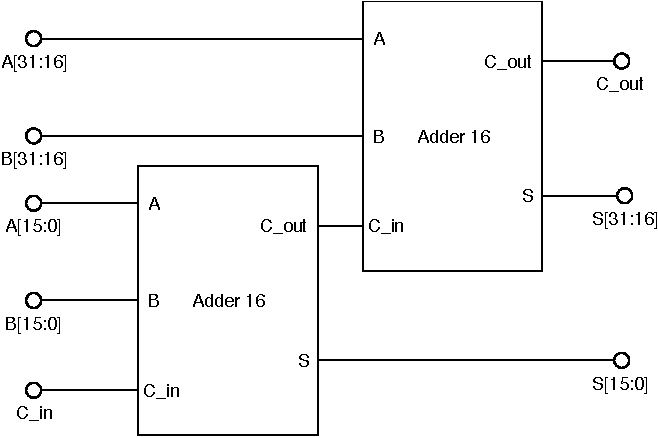
\includegraphics{../diagrams/alu/adder/adder_32.pdf}
        \caption{Logic diagram of the 32 bit adder}
    \end{figure}

    \paragraph{Testing}
    \hfill\\\\
    Due to the larger range of possible inputs, inputs are selected to include
    several base cases, as well as the maximum input value case. The inputs
    and expected outputs are as follows:

    \hfill\\
    \begin{tabular}{|c|c|c||c|c|}
        \hline
        A & B & Carry In & S & Carry Output
        \\\hline\hline
        10 & 10 & 1 & 21 & 0
        \\\hline
        1 & 0 & 1 & 2 & 0
        \\\hline
        4294967295 & 0 & 1 & 0 & 1
        \\\hline
        4294967295 & 4294967295 & 1 & 4294967295 & 1
        \\\hline
    \end{tabular}

    \begin{figure}[H]
        \centering
        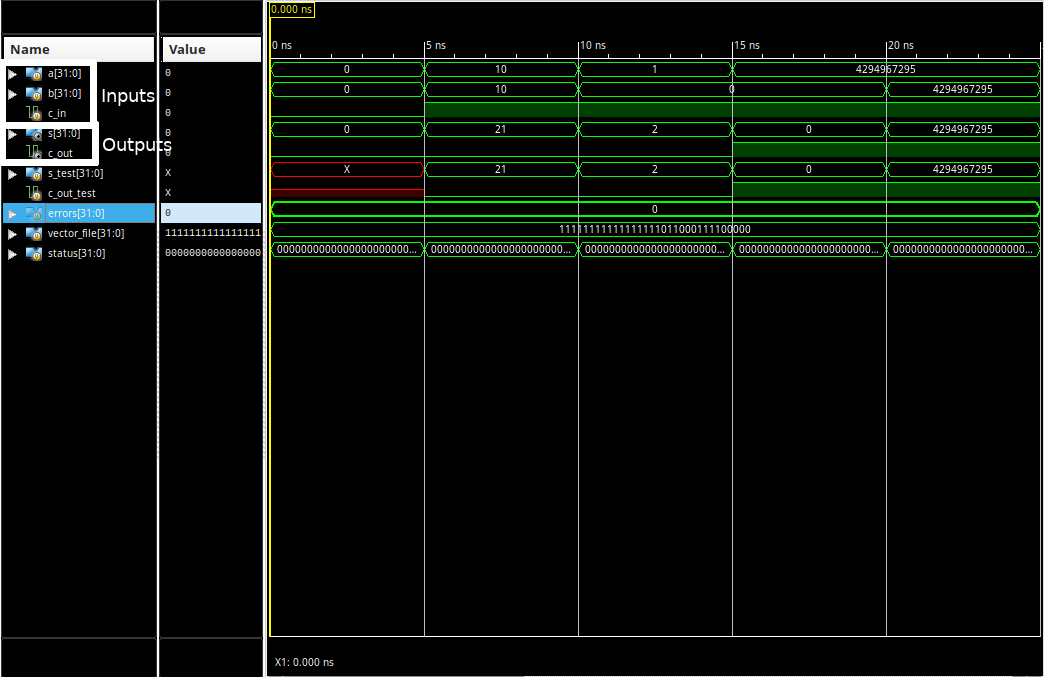
\includegraphics[width=0.9\paperwidth,center]{Screenshots/adder_32.png}
        \caption{Simulation output of 32 bit adder}
    \end{figure}

\end{document}